\chapter{模型设定}




\section{模型总体框架}

本研究构建了一个集成社交传播机制与行为金融模型的人工股票市场系统,旨在模拟网络暴力这一极端情绪事件如何通过社交网络影响投资者行为,并进一步扰动市场运行机制。整体模型以Agent-Based建模为基础,包含投资者行为模块、市场交易结构模块、网络暴力传播模块和实验分析模块四大核心组成部分,四者在系统中相互耦合,构成“情绪—行为—市场”闭环反馈结构。

在该系统中,投资者被建模为具有异质偏好、有限理性与社交关系的自主Agent,分为机构投资者与散户两类。两类Agent均可基于基本面预期、趋势信号与随机扰动做出交易决策,但在行为风格与受情绪影响程度上存在显著差异,特别是散户更易受到网络暴力影响而表现出沉默或激进等行为偏差。

市场交易结构采用连续双边报价(Continuous Double Auction, CDA)机制,通过订单簿系统撮合市价单与限价单形成成交价格。基础资产价格由布朗运动驱动,模拟市场的外部波动环境。所有Agent的交易意愿以订单形式提交至市场,经过撮合成交,最终影响市场价格演化与财富流动路径。

网络暴力传播模块在散户投资者之间建立社交网络,模拟在社交媒体语境下攻击性言论的传播过程。该模块引入攻击者、受害者、旁观者三类角色转化机制,并设计了情绪感染(正反馈)与系统治理(负反馈)机制。具体传播过程遵循以下逻辑:攻击者选择邻居中的异见者进行言语攻击,受害者若暴露程度超过阈值则转为沉默或反击者,同时系统可通过举报、监管干预或个体心理韧性成长抑制传播范围。

实验分析模块用于对模型结果进行系统分析,主要从两个角度进行分析:一是投资者群体的财富状态变化,二是市场的总体状态(如流动性、波动性等)。该模块通过对两类投资者(散户与机构)财富变化的追踪,分析网络暴力情绪如何影响投资者的财富分布;同时,分析市场的流动性、波动率等指标,探讨网络暴力是否对市场质量产生显著影响。实验分析模块通过对比不同情境下的结果,验证网络暴力对市场的实际影响。

模型整体运行流程如下:在每个仿真时间步,市场随机激活部分投资者进行决策;情绪传播模块并行更新网络暴力状态;投资者依据当前情绪状态、策略参数与市场信息做出交易决策;订单经由市场结构撮合成交;价格、资产与情绪状态更新,进入下一个时间步。通过多轮模拟与对比实验,可以观察网络暴力机制在投资者行为、市场稳定性与财富演化中的影响路径。


\begin{figure}[h]
    \centering
    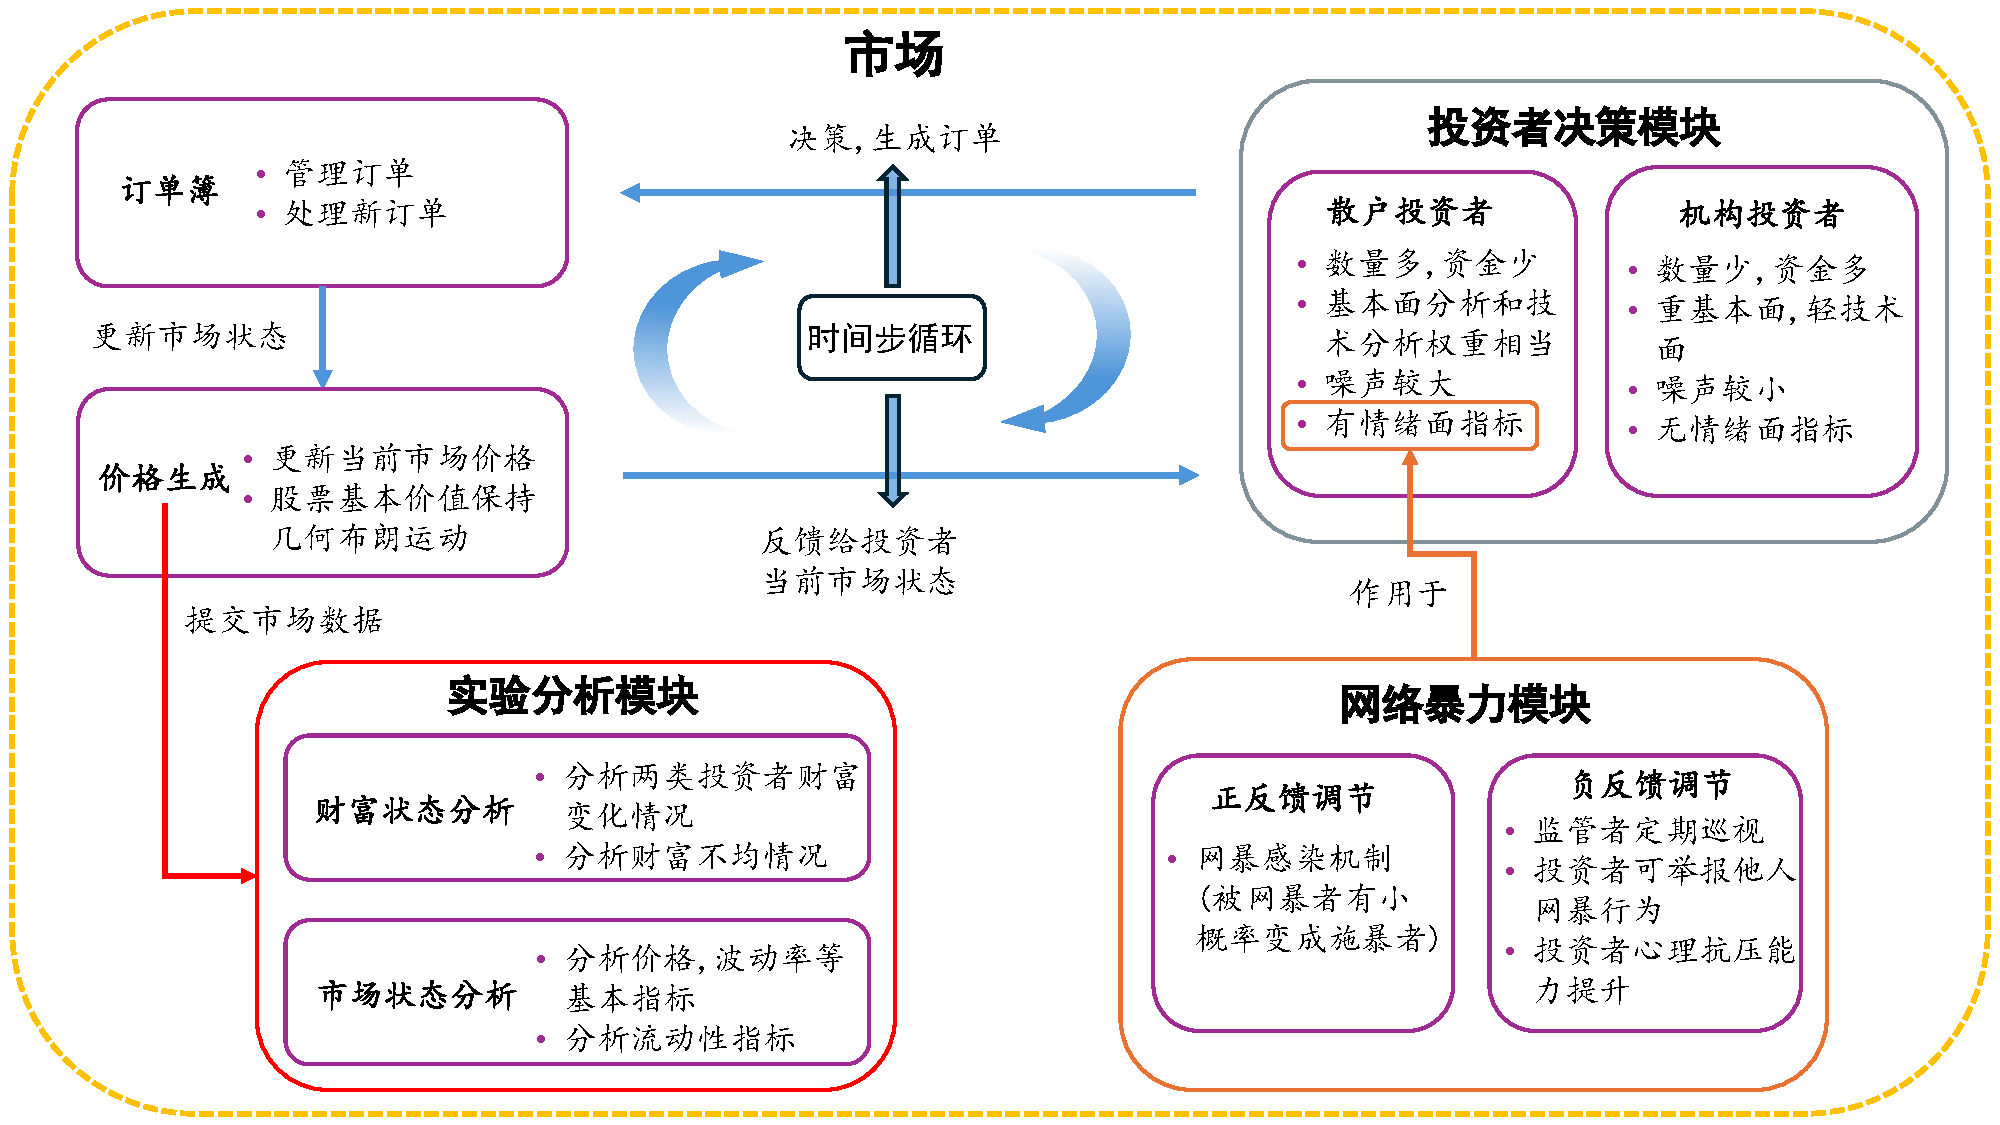
\includegraphics[width=0.8\textwidth]{image/3-1_structure.pdf}
    \caption{模型整体架构}
    \label{fig:architecture}
\end{figure}

图\ref{fig:architecture} 展示了模型的总体结构框架,四个核心子系统通过状态变量与行为函数实现交互,形成多层次、跨模块的系统性耦合。








\section{市场结构模块}

市场结构模块模拟了股票市场中的交易机制,特别是订单簿管理、订单匹配以及价格生成过程。本部分将首先讨论订单和订单簿的功能与实现,随后分析市场如何通过订单簿撮合机制生成价格并更新市场状态。

\subsection{订单与订单簿}


市场交易通过订单簿(Order Book)进行管理,订单簿包含市场上所有的买单和卖单,按照价格优先和时间优先的规则进行排列,并通过撮合机制完成交易。在本模型中,投资者可以提交两种类型的订单:市价单(Market Order)和限价单(Limit Order)。

市价单是指投资者希望以市场上当前最优价格立即成交的订单,买单市价单与当前最优卖单匹配,卖单市价单与当前最优买单匹配。限价单则是投资者愿意在特定价格或更好价格下买入或卖出资产的订单。限价单会根据价格优先和时间优先的规则排队,价格优先确保更高的买单和更低的卖单优先成交,时间优先则确保在价格相同的情况下,先提交的订单优先成交。

限价单的提交和撮合过程如下:

1. 买单限价单:在订单簿中,买单限价单按价格从高到低排列。只有当卖单的价格满足买单的价格时,买单才能成交。若价格相同,按时间优先规则进行撮合。

2. 卖单限价单:卖单限价单按价格从低到高排列,买单的价格需要等于或高于卖单的价格才会发生成交。若价格相同,按照提交时间优先。

限价单的核心是它为市场提供了深度,当市场价格变动时,挂单价格会进行相应的调整。只有当市场价格到达某个限价单的价格时,订单才会被执行。

另一方面,市价单与限价单的关系较为复杂,市价单会根据当前订单簿中的最优卖单(对于买单市价单)或最优买单(对于卖单市价单)立即执行。市价单的优先性使其能够快速成交,而限价单则在价格条件不满足时等待成交。若市价单的数量大于市场中最优对手单的数量,未成交的部分会转为限价单,继续在订单簿中等待匹配。

市场中的买单和卖单队列由订单簿进行管理。订单簿通过使用堆(heapq)数据结构实现对订单的优先级排序。买单按价格从高到低(负数价格)排序,卖单按价格从低到高排序,确保买卖双方能够根据最优价格进行交易。


表 \ref{tab:buy_orderbook} 展示了一个典型的买单订单簿示意表,其中包括了买单的订单编号、交易者ID、买入数量、价格、时间戳和订单状态等信息。



\begin{table}[htbp]
    \centering
    
    
    \begin{tabularx}{\textwidth}{@{} *{6}{>{\centering\arraybackslash}X} @{}}
    \toprule
    订单编号 & 交易者ID & 买入数量 & 价格 & 时间戳 & 订单状态 \\ \midrule
    1 & 101 & 100 & 99.95 & 1 & 待处理   \\
    2 & 102 & 200 & 99.90 & 2 & 待处理   \\
    3 & 103 & 150 & 99.85 & 3 & 已成交  \\
    4 & 104 & 100 & 99.80 & 4 & 待处理  \\
    5 & 105 & 50  & 99.75 & 5 & 已取消 \\ \bottomrule
    \end{tabularx}
    \caption{买单订单簿示意表}
    \label{tab:buy_orderbook}
\end{table}

在实际市场中,订单簿会随时间的推移动态变化,特别是当市场价格波动时,投资者提交的限价单会被重新排序,市价单则根据当前市场价格立即成交。每个时间步,模型会根据最新的市场状态和订单簿情况进行更新,形成价格和市场行为的反馈循环。





\subsection{价格生成机制与市场状态更新}

在本模型中,基础价格由几何布朗运动(Geometric Brownian Motion, GBM)生成,而市场价格则通过市场中的订单簿和交易活动动态生成。基础价格反映了市场资产的长期趋势和短期波动,而市场价格则是由市场参与者的交易行为和订单簿状况决定的。基础价格和市场价格的相互作用是市场价格动态更新的核心。

1. 基础价格生成

基础价格的生成依赖于几何布朗运动模型,这是金融市场中常用的价格生成模型。几何布朗运动模型的价格更新公式如下:

\begin{equation}
    p_{t+1} = p_t \exp\left( \mu \Delta t + \sigma \epsilon_t \sqrt{\Delta t} \right)
\end{equation}

其中,\( p_t \) 是当前价格,\( \mu \) 是漂移项,表示资产的长期趋势,\( \sigma \) 是波动率,表示价格的波动幅度,\( \epsilon_t \) 是标准正态分布的随机扰动项,\(\Delta t\) 是时间步长。

几何布朗运动能够模拟市场中常见的随机波动,反映资产价格的随机性和市场的不确定性。基础价格是市场中的理论价格,它不直接反映交易者的决策和市场供需情况,而是一个由宏观因素和市场波动性驱动的参考价格, 在本模型中是交易者进行基本面分析时的重要参照。

2. 市场价格生成

市场价格是由市场中的买单和卖单通过订单簿的撮合机制决定的。每个市场时间步,投资者通过市价单或限价单提交订单,市场则根据最优买单和最优卖单的价格进行撮合。当买单价格大于或等于卖单的最优价格时,订单会成交,成交价格即为市场价格。
如果在某一时间步没有成交,则市场价格将根据当前最优买单和最优卖单的价格更新,具体公式如下:

\begin{equation}
    \text{Market Price} = 
    \begin{cases} 
    \text{last\_price} & \text{如果上一时间步有交易发生} \\
    \frac{\text{best\_bid} + \text{best\_ask}}{2} & \text{如果上一时间步没有交易发生}
    \end{cases}
\end{equation}
在市场价格的生成过程中,市价单和限价单之间的相互作用起到了关键作用。市价单是根据当前市场最优对手单立即成交的订单,而限价单则需要在特定的价格范围内等待成交。市价单的成交价格通常会成为市场的最新价格,反映了市场供需的实时状况。





3. 市场状态更新

市场价格更新的基本过程如下:

- 市价单成交:市价买单会与当前最优卖单匹配,而市价卖单会与当前最优买单匹配。当市价单和限价单匹配时,成交价格即为最优买单或卖单的价格。
   
- 订单簿更新:每次成交后,订单簿中的相应订单会被移除,剩余的订单根据价格和时间优先规则重新排列。如果价格发生变化,订单簿将更新,确保挂单的顺序正确。

- 市场价格更新:市场成交价格会被用作当前市场的参考价格,并更新市场价格。通过对成交价格的跟踪,市场价格会反映出当前交易者的行为和市场的供需状况。

市场状态的更新不仅仅是价格的变化,还包括市场的流动性、深度和交易量等因素。在每个时间步,市场的流动性和深度都会随着订单簿的变化而更新。流动性反映了市场能够在不显著影响价格的情况下吸纳大规模交易的能力,而市场深度则表示在特定价格区间内存在的买单和卖单的数量。

市场的买卖价差(Bid-Ask Spread)可以通过以下公式计算:

\begin{equation}
    \text{Bid-Ask Spread} = \text{best\_ask} - \text{best\_bid}
\end{equation}

市场的深度表示市场中各个价格级别的买单和卖单的总数量。市场深度可以通过以下公式进行计算:

\begin{equation}
    \text{Market Depth} = \sum_{i=1}^{n} (\text{buy\_quantity}_i + \text{sell\_quantity}_i)
\end{equation}

其中,\( \text{buy\_quantity}_i \) 和 \( \text{sell\_quantity}_i \) 分别表示在档位 \( i \) 上的买单和卖单数量,\( n \)代表盘口档数(一般为5档)。市场深度可以反映市场的流动性,即在不显著影响价格的情况下能够吸纳的订单量。

